\section{An Example}\label{motivExample}

In this section we demonstrate our algorithm on small simple problem.
We use very simple query in our example, but it is classical context-free \textit{same-generation queries}~\cite{FndDB}, which is base for other context-free queries~\cite{GraphQueryWithEarley}.

Suppose that you are student in a School of Magic.
It is your first day at School, so navigation in the building is a problem for you.
Fortunately, you have a map of the building (fig.~\ref{input}) and additional knowledge about building construction:
\begin{itemize}
  \item there are towers in the school (depicted as nodes of the graph in your map);
  \item towers can be connected by one-way galleries (represented as edges in your map);
  \item galleries have a ``magic'' property: you can start from any floor, but by following each gallery you either end up one floor above (edge label is `a'), or one floor below (edge label is `b'). 
\end{itemize}

\begin{figure}[h]
    \begin{center}
	\centering
    \begin{subfigure}[b]{0.45\textwidth}
        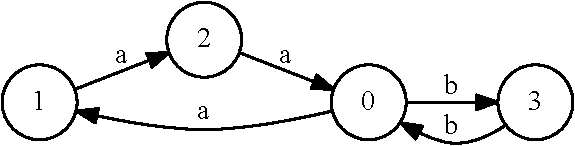
\includegraphics[width=\textwidth]{dot/input.pdf}
        \caption{The map of School (input graph $M$)}
        \label{input}        
		\vspace{1cm}
	\end{subfigure}
	~	
	\begin{subfigure}[b]{0.45\textwidth}
   \[
\begin{array}{rl}
   0:& S \rightarrow a \ S \ b \\
   1:& S \rightarrow Middle \\
   2:& Middle \rightarrow a \ b
\end{array}
\]
   \caption{Grammar $G_1$ for language $L=\{a^n b^n; n \geq 1\}$ with additional marker for the middle of a path}
   \label{grammarG}        
	\end{subfigure}
    \end{center}
\caption{An example: input graph and grammar}
\label{exampleData}
\end{figure}


You want to find a path from your current position to the same floor in another tower. 
Map with all such paths can help you.
But orienteering is not your forte, so it would be great if the structure of the paths were as simple as possible and all paths had additional checkpoints to control your rout.

It is evident that the simplest structure of required paths is $\{ab, aabb, aaabbb, \dots\}$.
In terms of our definitions, it is necessary to find all paths $p$ such that $\Omega(p) \in \{a^n b^n, n \geq 1\}$ in the graph $M=(\{0;1;2;3\},E,\{a;b\})$ (figure~\ref{input}).

Unfortunately, language $\mathcal{L} = \{a^n b^n; n \geq 1\}$ is not regular which restricts the set of tools you can use. 
Another problem is the infinite size of solution, but, being incapable to comprehend an infinite set of paths, you want to get a finite map.  
Moreover, you want to know structure of paths in terms of checkpoints.

We are not aware of any existing tools which can solve this problem, thus we have created such tool.
Let us show how to get a map which helps to navigate in this strange School.

Fortunately, the language $\mathcal{L} = \{a^n b^n; n \geq 1\}$ is a context-free language and it can be specified with context-free grammar. 
The fact that one language can be described with multiple grammars allows to add checkpoints: additional nonterminals can mark required parts of sentences.
In our case, desired checkpoint can be in the middle of the path.
As a result, required language can be specified by the grammar $G_1$ presented in figure~\ref{grammarG}, where $N = \{s; \text{\textit{Middle}}\}$, $\Sigma = \{a; b\}$, and $S$ is a start nonterminal.

Now, let us show that SPPF can be a solution for this problem.
SPPF for data from example is presented in figure~\ref{SPPF}.
Each terminal node corresponds to the edge in the input graph: for each node with label $(v_0, T, v_1)$ there is $e\in E: e=(v_0,T,v_1)$.
Extensions stored in SPPF nodes allow us to check whether path from $u$ to $v$ exists and to extract it by SPPF traverse. 

\begin{figure*}[ht]
    \begin{center}
    \centering
    \begin{subfigure}[b]{0.3\textwidth}
         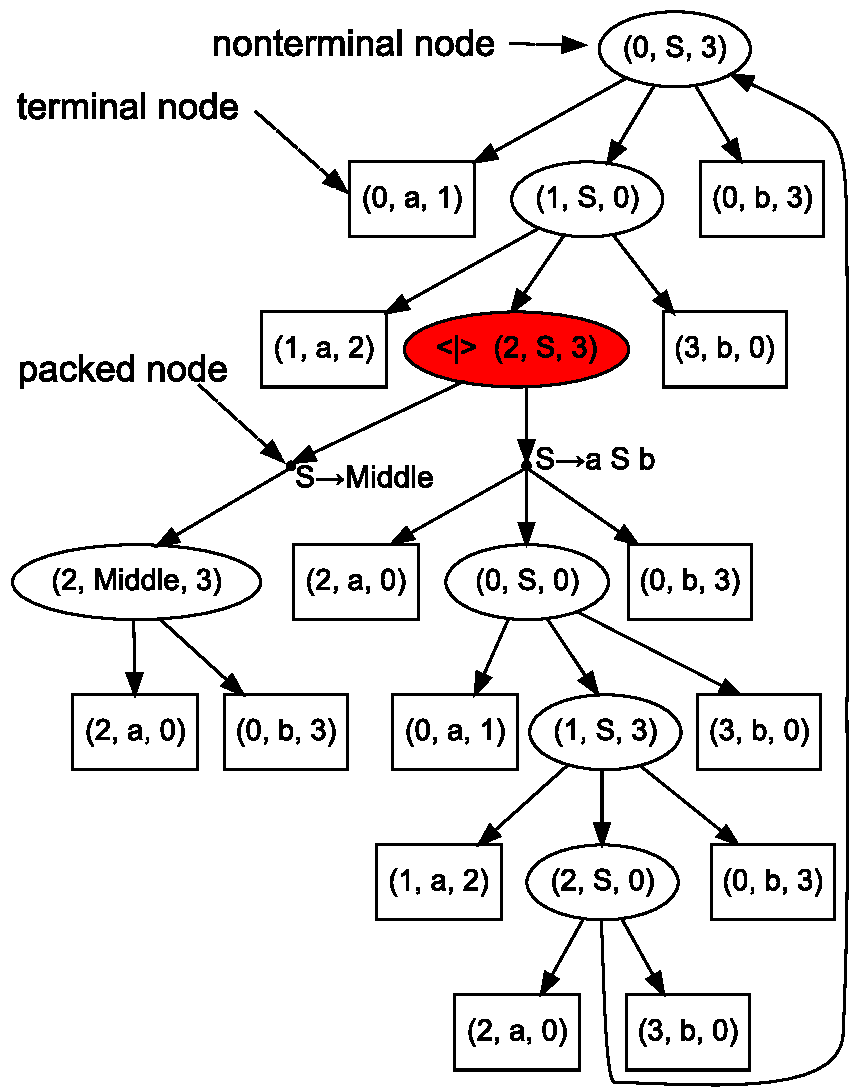
\includegraphics[width=\textwidth]{dot/AnBn.pdf}
        \caption{Result SPPF}
        \label{SPPF}        
    \end{subfigure}
    ~
    \begin{subfigure}[b]{0.3\textwidth}
        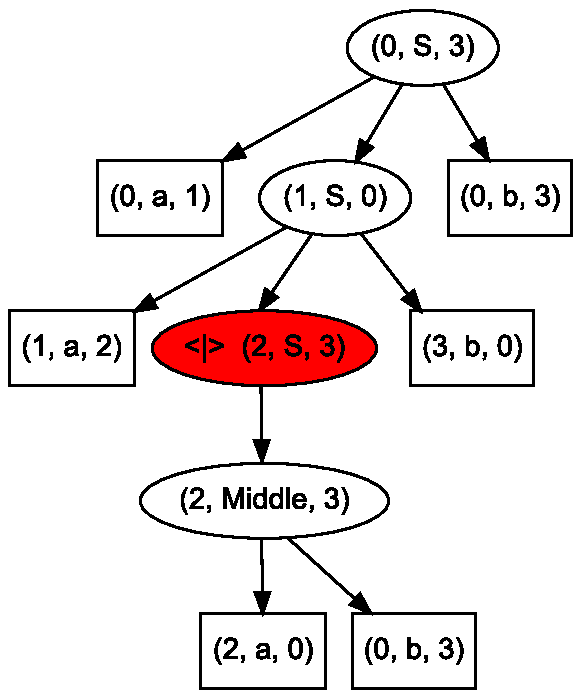
\includegraphics[width=\textwidth]{dot/AnBn_2.pdf}
        \caption{Derivation tree for $p_0$}
        \label{tree1}        
    \end{subfigure}
    ~
    \begin{subfigure}[b]{0.3\textwidth}
        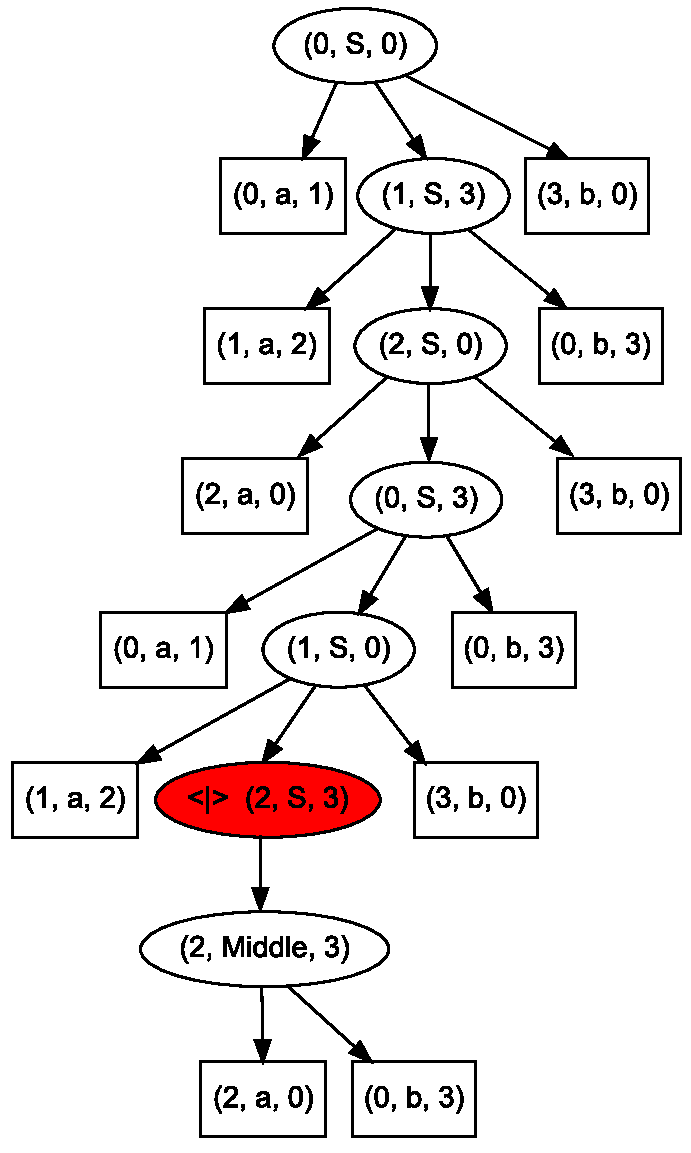
\includegraphics[width=\textwidth]{dot/AnBn_1.pdf}
        \caption{Derivation tree  for $p_1$}
        \label{tree2}        
    \end{subfigure}
    \caption{SPPF and examples of trees for specific paths for data from example (fig~\ref{exampleData}). Presented version does not contains redundant nodes, and we duplicate terminal nodes only for figure simplification.
    We use filled shape and label of form $(<\mkern-11mu | \mkern-11mu> (i, N, j))$ for nonterminal node to denote that there are multiple derivations from nonterminal $N$ for substring $\omega[i..j-1]$.	
	%\\
	%$p_0=\{(0,a,1);(1,a,2);(2,a,0);(0,b,3);(3,b,0);(0,b,3)\}$  \\
    %$p_1=\{(0,a,1);(1,a,2);(2,a,0);(0,a,1);(1,a,2);(2,a,0);(0,b,3);(3,b,0);(0,b,3);\\(3,b,0);(0,b,3);(3,b,0)\}.$
}
    \label{sppfSample}
    \end{center}                
\end{figure*}

As an example of derivation structure usage, we can find a middle of any path in example simply by finding correspondent nonterminal \textit{Middle} in SPPF.
So we can find out that there is only one (common) middle for all results, and it is a vertex with $id = 0$.

Lets find paths $p_i$ such that $S {\xRightarrow[G_1]{}}^{*} \Omega(p_i)$ and $p_i$ starts from the vertex $0$.
To do this, we should find vertices with label $(0, S, \_)$ in SPPF.
(There are two vertices with such labels: $(0, S, 0)$ and $(0, S, 3)$.)
Then let us to extract corresponded paths from SPPF.
There is a cycle in SPPF in our example, so there are \textbf{at least} two different paths: $p_0=\{(0,a,1);(1,a,2);(2,a,0);(0,b,3);(3,b,0);(0,b,3)\}$ and 
$
p_1=\{(0,a,1);(1,a,2);(2,a,0);(0,a,1);(1,a,2);(2,a,0);(0,b,3);(3,b,0);(0,b,3);\\(3,b,0);(0,b,3);(3,b,0)\}.
$ Trees for these paths are presented in figures~\ref{tree1} and~\ref{tree2} respectively.
%\end{align*}

We demonstrate that SPPF which was constructed by described algorithm can be useful for query result investigation. 
But in some cases explicit representation of matched subgraph is preferable, and required subgraph may be extracted from SPPF trivially by its traversal.
